%!TEX root=../../main.tex
\section{Datenschnittstelle und Webseitenlogik}
\label{chapter:implementierung-datenschnittstelle}
\subsection{Webseitenlogik}
Wie in \autoref{sec:webseitenlogik} beschrieben, wird die Webseitenlogik größtenteils von einem \textit{Manager} übernommen.

\subsubsection{Navigation}
\label{sec:navigation}
Die Unterseiten werden in den \textit{Manager} geladen und je nach Gebrauch angezeigt. Dafür gibt es eine Variable im \textit{Manager}, welche dafür sorgt, dass nur eine Komponente auf einmal angezeigt werden kann. Die Komponente wird gewechselt, indem die folgende Funktion aufgerufen wird:
\begin{code}{js}
	changeComponent(
	component,
	back = true,
	application = null,
	escortsdata = null
	) {
		switch (component) {
			case "Login":
			this.change("Login", back);
			this.deleteCookie();
			break;
			
			case "Index":
			this.change("Index", back);
			break;
			
			case "ApplicationView":
			this.loadApplication(application);
			this.change("ApplicationView", back);
			break;
			
			case "Escorts":
			this.loadEscortsData(escortsdata);
			this.change("Escorts", back, false);
			break;
			
			// [Weitere Unterseiten]
		}
	}
\end{code}
\captionof{listing}[Funktion Anzeige ändern]{Funktion zum Ändern der angezeigten Komponente}~\\
\newpage
Diese Funktion besteht hauptsächlich aus einer Verzweigung, die entscheidet, welche Seite angezeigt werden soll.
Des Weiteren gibt es bei manchen Komponenten den Zusatz einer \textit{load}-Funktion, welche Daten für die jeweilige Komponente vorbereitet bzw. berechnet.

Die referenzierte \textit{change}-Funktion übernimmt das tatsächliche Ändern der Variable:
\begin{code}{js}
	change(page, back = true, cookie = true) {
		this.currentComponent = page;	// Es wird die angezeigte Seite verändert
		window.scrollTo(0, 0);	// Es wird zum Anfang der Seite gegangen
		if (back) {
			if (window.history.state !== page) {
				window.history.pushState(page, null);	// Es wird die übergebene Seite in die History des Browsers geschrieben
			}
		}
		if (cookie) {
			this.setCookie(page);	// Es wird der Cookie gesetzt
		}
\end{code}
\captionof{listing}[Funktion Managment der \textit{Cookies} und \textit{History}]{Funktion für das Managment der \textit{Cookies} und \textit{History} des Browsers}~\\
Hier werden nicht nur die angezeigte Seite verändert, sondern auch je nach Parameter die \textit{Cookies} sowie die \textit{History} des Browsers gesetzt.\\
Die beschriebenen Funktionen müssen von den Komponenten aufgerufen werden können. Deswegen hört der \textit{Manager} auf Signale der Unterseiten, falls diese die Seite geändert werden soll. Dies wird mittels VueJS erledigt, da das Framework hierfür bereits Funktionen implementiert hat:
\begin{code}{js}
	v-on:change-component="changeComponent"
	// Es wird auf das Signal change-component gehört und die Funktion changeComponent aufgerufen
\end{code}
\captionof{listing}[Event Handling]{Event Handling mittels v-on}~\\
Die Codezeile wird beim Aufruf der Unterseite im \textit{Manager} hinzugefügt.\\
Die beschriebenen Signale werden von den Unterseiten mittels folgendem Code bzw. folgender Funktion gesendet:
\begin{code}{js}
	changeComponent(component, back, application, escortsdata) {
		this.$emit("change-component", component, back, application, escortsdata);
	}
\end{code}
\captionof{listing}[Signal senden]{Ein Signal an die übergeordnete Komponente senden}~\\
Hier wird durch \textit{this.\$emit()} ein Befehl an die übergeordnete Seite gesendet.
\newpage
\subsubsection{Komponenten}
Die Komponenten der Unterseiten werden, wie im vorherigen Kapitel beschrieben, in den \textit{Manager} eingebunden. Dies wird mit dem Importieren, dem Laden und der Implementierung der Komponente umgesetzt.
Das Importieren erfolgt mit folgendem Code:
\begin{code}{html}
	<script>
	import ApplicationView from "@/components/ApplicationView.vue";
	// [Weitere Imports]
	
	export default {
		components: {
			ApplicationView
			// [Weitere Komponenten]
		}
	}
</script>
\end{code}
\captionof{listing}[Importieren und Laden einer Komponente]{Umsetzung des Importieren und Laden einer Komponente im \textit{Manager}}~\\
In dem Code werden von \textit{@/components/} die einzelnen Komponenten geladen. Aufgrund der Verwendung von \textit{@} wird das Angeben des vollen Pfades nicht mehr benötigt, da dies auf den relativen Pfad der Softwarestruktur zeigt.
\newpage
Die Komponente muss noch im \textit{Manager} angezeigt werden. Dies wird im \textit{Template} des \textit{Managers} mit folgendem Code umgesetzt:
\begin{code}{html}
<template>
	<div class="home">
		<Login
			v-if="currentComponent == 'Login'"
			v-on:change-component="changeComponent"
			v-bind:url="url"
			v-bind:token="token"
			v-bind:forward="forward"
			v-on:requestAnswer="useCookie"
			v-bind:cookieset="cookies"
			v-on:login="login"
		/>
		<Index
			v-if="currentComponent == 'Index'"
			v-on:change-component="changeComponent"
			v-bind:url="url"
			v-bind:token="token"
			v-bind:admin="admin"
			v-bind:user="user"
		/>
		<ApplicationView
			v-if="currentComponent == 'ApplicationView'"
			v-on:change-component="changeComponent"
			v-bind:url="url"
			v-bind:token="token"
			v-bind:appid="appid"
			v-bind:user="user"
		/>
		<!-- Weitere Komponenten -->
	</div>
</template>
\end{code}
\captionof{listing}[Anzeige der Komponenten]{Anzeigen der Komponenten im \textit{Manager}}~\\
Im Code wird nicht nur die Komponente angezeigt, sondern auch Daten an die Komponenten gebunden.\\
\textit{v-if}-Attribute sorgen dafür, dass das Rendern nur unter der angegebenen Bedingung erfolgt. Die Komponente wird nur angezeigt, wenn die Variable \textit{currentComponent} den Namen einer Komponente annimmt.\\
\textit{v-bind}-Attribute binden Daten von der übergeordneten Komponente in die eingebundene Komponente ein. Bei dem Beispiel \textit{v-bind:cookieset=''cookies''} wird an die \textit{Login}-Komponente ein Attribut \textit{cookieset} mit dem Wert von der Variable \textit{cookies} mitgegeben.
Diese Attribute können mit folgendem Code aufgefangen und in diesen eingebundenen Komponenten verwendet werden:
\begin{code}{html}
		props: ["url", "forward", "cookieset"]
\end{code}
\captionof{listing}[Auffangen übergebener Variablen]{Auffangen übergebener Variablen in einer untergeordneten Komponente}~\\
In dem Code werden die übergebenen Variablen, welche in der übergeordneten Komponente definiert worden sind, aufgefangen. Diese können als normale Variablen verwendet werden.
\newpage
\subsubsection{Seite nicht gefunden}
Wie in \autoref{sec:not_found} beschrieben wird, wird der Benutzer bei Eingabe eines falschen Links auf eine Seite weitergeleitet. Dazu wird der \textit{Vue-Router} so eingestellt, dass jeder Link, außer dem Hauptlink zur eigentlichen Webseite, auf die beschriebene Seite weitergeleitet wird. Die Routen des Routers sind wie folgt aufgebaut:
\begin{code}{js}
// Imports für die Komponenten
import Vue from "vue";
import VueRouter from "vue-router";
import Home from "../views/Home.vue";
import PageNotFound from "../components/PageNotFound.vue";

Vue.use(VueRouter);		// Sagt dem Projekt, dass es den Router verwenden soll

const routes = [
{
	path: "/",					// Der Pfad, der von dem Benutzer eingegeben wird
	name: "Home",				// Der Name des Pfades
	component: Home,			// Die Komponente, welche angezeigt werden soll
	props: { pathing: "base" }	// Variablen, welche an die Komponente gesendet werden sollen
},
{
	path: "/viewer",
	name: "Viewer",
	component: Home,
	props: route => ({ query: route.query.uuid })	// Die ID des Antrags, welcher betrachtet werden möchte
},
{
	path: "*",				// Fasst alle nicht erwähnten Routen zusammen
	name: "NotFound",
	component: PageNotFound
}
];
const router = new VueRouter({
	mode: "history",
	base: process.env.BASE_URL,
	routes
});

export default router;
\end{code}
\captionof{listing}[Pfadverwaltung]{Router, welcher die Pfade der Software verwaltet}~\\

Wird ein Link eingegeben, welcher nicht ''/'' oder ''/viewer'' entspricht, so wird die \textit{PageNotFound}-Komponente geladen und somit dem Benutzer mitteilt, dass der eingegebene Link nicht funktioniert.
\subsubsection{Antrag-Viewer}
\label{sec:antrag_viewer}
Der \textit{Antrag-Viewer} wird über den Link \textit{/viewer} aufgerufen. Dies führt dazu, dass der Benutzer auf eine Seite weitergeleitet wird, auf der er die ID eines Antrags eingeben kann.
\begin{figure}[H]
	\centering
	
\includegraphics[width=1\linewidth]{images/rfoster_implementierung/antrag_viewer}
	\caption[Webseite \textit{Antrag-Viewer}]{Die \textit{Antrag-Viewer} Seite der Webseite}
	\label{fig:antragviewer}
\end{figure}

Sollte der Benutzer nicht angemeldet sein, so wird er zuerst auf die \textit{Login}-Seite weitergeleitet, bevor er die ID des Antrags eingeben kann. Sollte der eingegebene Link bereits den Parameter \textit{uuid} besitzen, wird der Benutzer auf die Antragsansichtsseite weitergeleitet, sofern dieser angemeldet ist. Ansonsten wird der Benutzer zuerst auf die \textit{Login}-Seite weitergeleitet.
\begin{code}{js}
	{
		// Die Route des Antrag-Viewers
		path: "/viewer",
		name: "Viewer",
		component: Home,
		props: route => ({ query: route.query.uuid }) // Der Parameter in der URL
	},
\end{code}
\captionof{listing}[Route für den \textit{Antrag-Viewer}]{Route für den \textit{Antrag-Viewer} mit Parametern}~\\
Es wird die Home-Komponente (der \textit{Manager}) aufgerufen, da dieser das Verarbeiten der URL und das Weiterleiten auf die \textit{Login}- und Antragsansicht übernimmt.
\newpage
\subsubsection{Features}
Die Features in \autoref{sec:feature} wurden folgendermaßen implementiert.

\paragraph{Zuletzt besuchte Seite der Webseite}~\\
Beim Laden der Webseite wird mithilfe von \textit{Cookies} auf die zuletzt besuchte Seite navigiert. Dazu wird bei jeder Navigation, wie in \autoref{sec:navigation} beschrieben, der \textit{Cookie} gesetzt. Dieser wird beim Laden der Webseite ausgelesen und es wird, falls der \textit{Cookie} gesetzt ist, auf die gespeicherte Seite navigiert.
\begin{code}{js}
	if (this.checkCookie()) {		// Abfrage, ob ein Cookie vorhanden ist
		this.useCookie(true);		// Sofern ein Cookie vorhanden ist, hat der Benutzer bereits die Cookies für diese Webseite akzeptiert
		var c = this.getCookie();	// Die Informationen des Cookies werden ausgelesen
		if (c == this.generateState(window.history.state)) {	// Falls die zuletzt besuchte Seite die gleiche ist, wie die aktuelle Seite, so wird kein neuer Eintrag in der History generiert
			this.changeComponent(c, false);
		} else {
			this.changeComponent(c);
		}
	} else {
		// Falls kein Cookie gesetzt ist, wird der Benutzer auf die Login-Seite weitergeleitet
		this.changeComponent("Login");
	}
\end{code}
\captionof{listing}[Navigation zuletzt besuchte Seite]{Navigation auf die zuletzt besuchte Seite}~\\

\paragraph{Browser-Pfeile}~\\
Die Browser-Pfeile navigieren durch die \textit{History} des Browsers. Da die Webseite ein One-Pager ist, muss das Schreiben in die \textit{History} selbst übernommen werden. Dies wird durch den folgenden Code umgesetzt:
\begin{code}{js}
window.addEventListener("popstate", e => {			// Es wird ein Listener auf die Webseite gesetzt
	if (this.generateState(e.state) === "Escorts") {	// Dies ist eine extra Abfrage, welche verhindert auf die Escorts-Seite zu gelangen.
		this.changeComponent("School", false);
	} else {
		this.changeComponent(this.generateState(e.state), false);	// Es wird auf die Unterseite navigiert.
	}
});
\end{code}
\captionof{listing}[Unterstützung Browser-Pfeile]{Unterstützung der Browser-Pfeile}~\\
Das Hinzufügen der einzelnen \textit{Histories} für die jeweiligen Unterseiten wird in \autoref{sec:navigation} beschrieben.
\newpage
\subsection{Daten laden \& Befehle senden}
Das Laden, sowie das Befehle senden, wird mittels \Gls{axios} umgesetzt. Es gibt vier Arten der Anfragen per \Gls{axios}, welche verwendet werden. \textit{Get} (Anfrage von Daten), \textit{put} (Aktualisieren von Daten), \textit{post} (Erstellen von Daten) und \textit{delete} (Löschen von Daten). Mit folgender Struktur können Daten geladen werden von dem Backend, bzw. der REST-Schnittstelle:
\begin{code}{js}
	axios.get(this.url + "/getNews", {
		headers: {
			Authorization: "Basic " + this.token
		}
	}).then(response => {
		switch(response.status) {
			case 200:
				this.news = this.cutNews(response.data); // Hier werden die Neuigkeiten aus der Anfrage in die Startseite geladen
				break;
			case 401:
				// Hier wird auf den Fehlercode 401 reagiert
				break;
			default:
				// Hier wird dem Benutzer angezeigt, dass ein Fehler aufgetreten ist
				break;
		}
	}
	});
\end{code}
\captionof{listing}[Laden von Neuigkeiten]{Laden der Neuigkeiten auf der Startseite}~
\newpage
Unter der Bedingung, dass die erste Anfrage den Fehlercode \textit{401} zurückgibt, wird eine Anfrage an das Backend gesendet, um die Sitzung des Nutzers zu aktualisieren. Dies wird mit folgendem Code umgesetzt:
\begin{code}{js}
	axios.post(this.url + "/login/refresh", {
		headers: {
			Authorization: "Basic " + this.refresh_token
		}
	}).then(resp => {
		switch (resp.status) {
			case 201:
				this.$emit"updateToken", resp.data.access_token, resp.data.refresh_token);
				// Die Anfrage wird erneut durchgeführt
				break;
			default:
				this.$emit("logout"); // Der Benutzer wird vom System abgemeldet
				break;
			}
		}
	});
\end{code}
\captionof{listing}[Sitzung aktualisieren]{Anfrage um Sitzung des Nutzers zu aktualisieren}~\\
Bei erfolgreicher Erneuerung der Sitzung, wird die anfangs durchgeführte Anfrage erneut gesendet. Diese reagiert, bis auf die fehlende Behandlung des Fehlercodes \textit{401}, ident, wie die originale Anfrage.
\newpage
\subsection{Anmelden}
Der Benutzer kann sich auf einer Anmeldeseite anmelden, um das System verwenden zu können. Dazu werden die Anmeldedaten des Benutzers an das Backend gesendet. Um sich anmelden zu können, müssen die \textit{Cookies} akzeptiert werden. Sollten sie nicht akzeptiert werden, ist es nicht möglich den Dienst zu verwenden.
Sobald der Benutzer erfolgreich angemeldet ist, wird dieser auf die Hauptseite weitergeleitet.
\\
\begin{code}{js}
axios.post(this.url + "/login", {	// Sendet ein POST-Anfrage an das Backend
	username: this.email,	// Die eingegebene E-Mail Adresse
	password: this.password // Das eingegebene Passwort
}).then(response => {
	var data = response.data
	// Es werden die Daten aus der Anfrage an den Manager gesendet, damit eine valide Sitzung erstellt wird.
})
\end{code}
\captionof{listing}[Umsetzung Login]{POST-Anfrage für den Login}~\\

\subsubsection{Spezielle Situationen}
In besonderen Fällen, wie in \autoref{sec:antrag_viewer} beschrieben, wird der Benutzer nicht auf die Hauptseite weitergeleitet, sondern auf den \textit{Antrag-Viewer} oder auf die \textit{Antrag-Ansicht}.
\begin{code}{js}
switch (this.forward.name) {	// Es wird entschieden, auf welche Unterseite navigiert werden soll
	case "ApplicationSearch":	// Es wird auf den Antrag-Viewer navigiert
	this.$emit("change-component", this.forward.name);
	break;
	case "ApplicationView":	// Es wird auf die Antrag Ansicht navigiert
	this.$emit(
	"change-component",
	this.forward.name,
	true,
	this.forward.id
	);
	break;
	default:	// Es wird auf die Hauptseite navigiert
	this.$emit("change-component", "Index");
	break;
}
\end{code}
\captionof{listing}[Login Weiterleitung]{Weiterleitung nach erfolgreichem Anmelden}~\\
\subsubsection{Passwort vergessen}
Da \textit{Refundable} die Anmeldedaten von \textit{LDAP} verwendet, wird der Benutzer auf \href{https://owa.tgm.ac.at}{OWA} weitergeleitet, wenn auf ''Passwort vergessen'' gedrückt wird.
\newpage
\subsection{Abmelden}
Wird auf den ''Abmelden''-Knopf gedrückt, wird ein Anfrage mit dem derzeit aktiven Token an das Backend gesendet, um den Authentifizierungstoken zu terminieren. Dies bedeutet, dass der Benutzer keinen validen Token mehr besitzt und auf die \textit{Login}-Seite weitergeleitet wird.
\begin{code}{js}
axios.post(this.url + "/logout", {	// Sendet ein POST-Anfrage an das Backend
	headers: { Authorization: this.token }	// Der Token des Benutzers
})
.then(response => {
	if (response.status === 200) {	// Falls die Anfrage erfolgreich war
		this.token = "";
		this.refresh_token = "";
		this.deleteCookie();
		this.changeComponent("Login");	// Es werden die Tokens und Cookies gelöscht und der Benutzer wird auf die Login-Seite weitergeleitet.
	}
});
\end{code}
\captionof{listing}[Anfrage Abmelden]{Gesamte Anfrage für das Abmelden}~\\
\newpage
\subsection{Antrag erstellen}
Ein Antrag kann von jedem Lehrer, der im System angemeldet ist, erstellt werden. Dazu wird auf die \textit{Antrag erstellen}-Unterseite navigiert, bei der der Benutzer aussuchen kann, ob er eine Schulveranstaltung, Fortbildung oder einen anderen Antrag erstellen möchte. Auf diesen Unterseiten werden die notwendigen Informationen vom Benutzer in die Eingabefelder eingegeben. Diese Informationen werden in ein \textit{JSON}-Objekt gegeben und an das Backend gesendet.
\\
In den folgenden Codebeispielen werden oft die Befehle \textit{returnString}, \textit{returnBoolean} und \textit{returnValue} verwendet. Diese dienen dazu die Datentypen auf die des Backends anzupassen. 
\subsubsection{Schulveranstaltung}
\paragraph{Allgemeine Informationen}~\\
Im ersten Schritt, werden allgemeine Informationen der Schulveranstaltung eingegeben.
\begin{figure}[H]
	\centering
	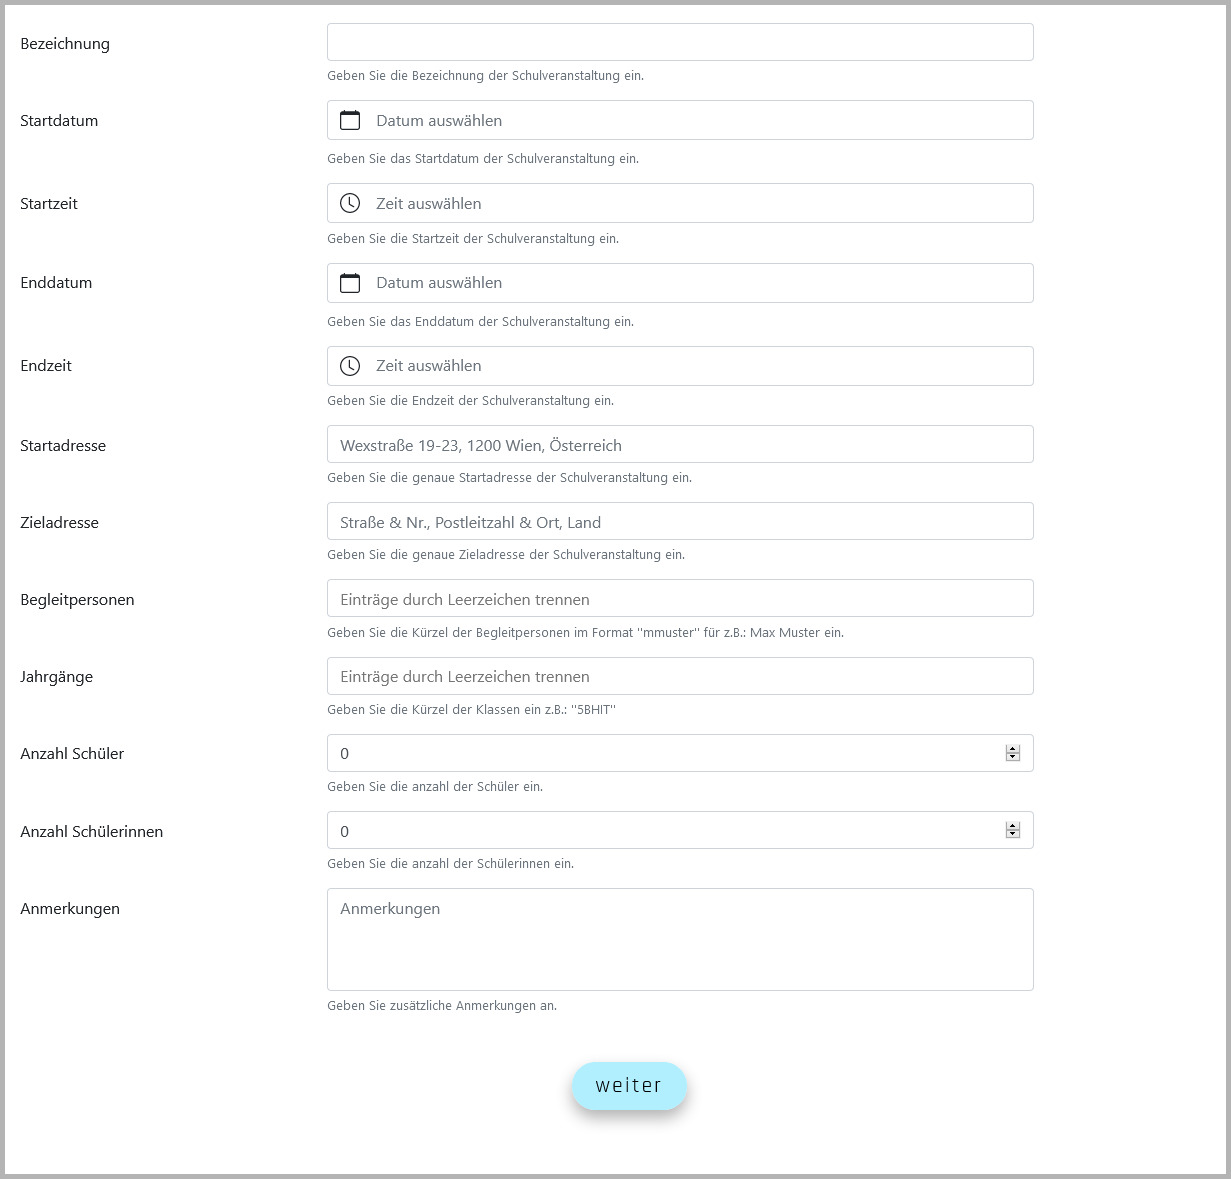
\includegraphics[width=1\linewidth]{images/rfoster_implementierung/schoolgeneral}
	\caption[Schulveranstaltung]{Eingabefelder für allgemeine Informationen einer Schulveranstaltung}
	\label{fig:schoolgeneral}
\end{figure}
\paragraph{Informationen zu Begleitlehrern}~
\label{code_submit_data}~\\
Nach der Eingabe aller allgemeinen Informationen wird der Benutzer nach dem Drücken des ''weiter''-Knopfes auf eine weitere Unterseite weitergeleitet. Auf dieser können Informationen zu den im vorherigen Schritt angegebenen Begleitlehrern angegeben werden.
\begin{figure}[H]
	\centering
	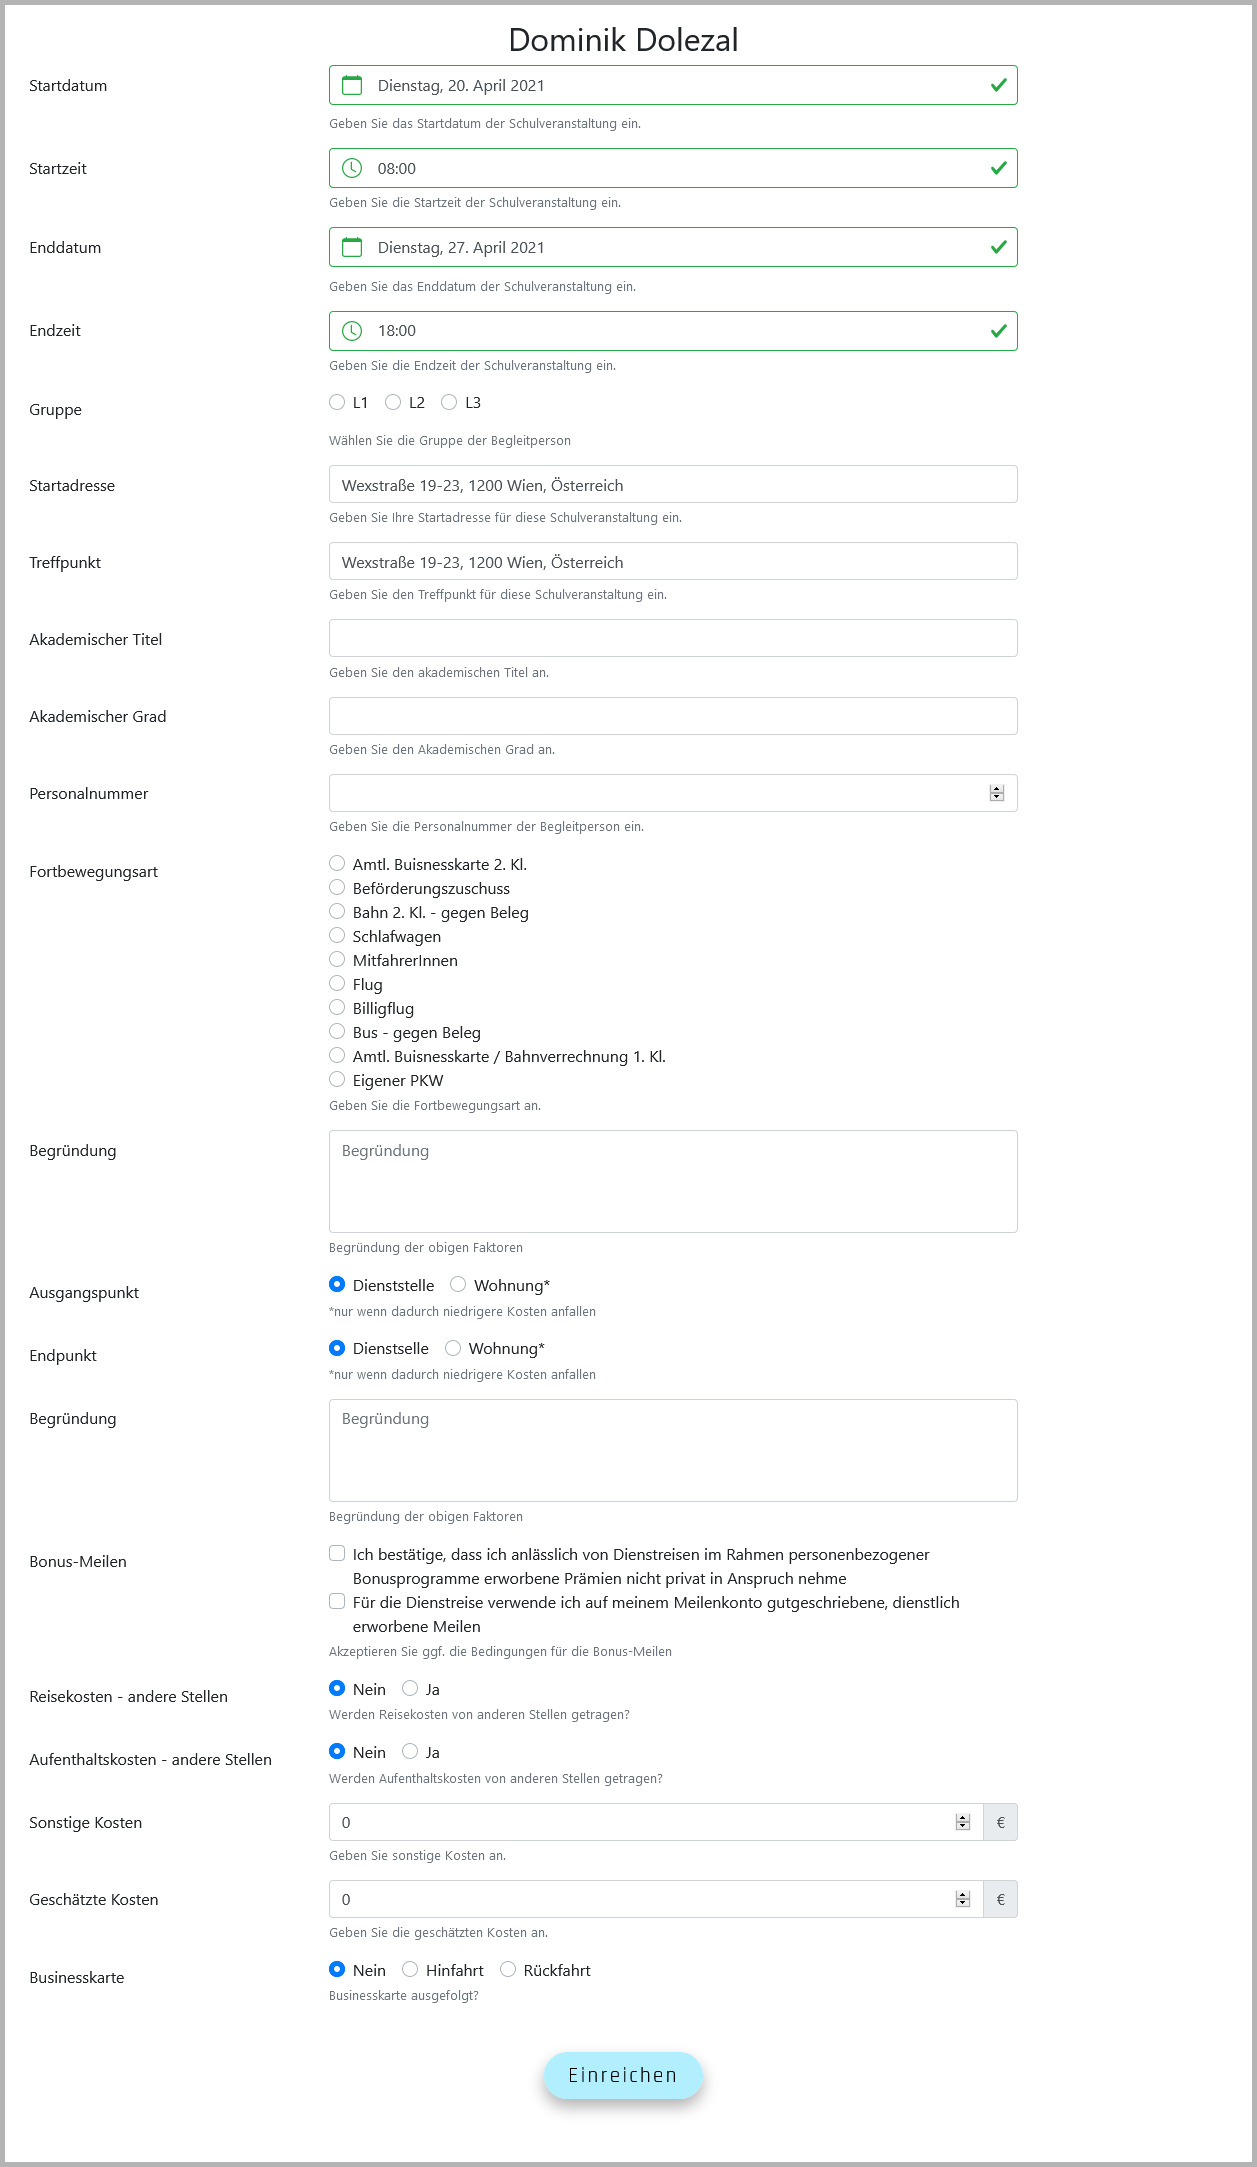
\includegraphics[width=0.7\linewidth]{images/rfoster_implementierung/escorts}
	\caption[Schulveranstaltung 2]{Eingabefelder für Informationen von Begleitlehrern}
	\label{fig:escorts}
\end{figure}
\newpage
Nachdem die Seite bearbeitet worden ist, kann auf den Knopf ''Einreichen'' gedrückt werden. Sobald der Knopf gedrückt worden ist, wird das \textit{JSON}-Objekt mit allen Informationen, die eingegeben worden sind, erstellt und an das Backend gesendet.
\begin{code}{js}
var data = {		// Das JSON-Objekt mit allen Informationen
	Name: this.returnString(this.escorts.description),	// Der Name des Antrags
	Kind: 0,	// Der Typ des Antrags (0 = Schulveranstaltung)
	MiscellaneousReason: this.returnString(""),			// Nicht benötigt, da es eine Schulveranstaltung ist
	Progress: 1,	// Der Fortschritt ist standardmäßig auf 1 gesetzt
	StartTime: this.setTimezone(	// Die Startzeit des Antrags
	new Date(this.escorts.startDate + "T" + this.escorts.startTime)
	),
	EndTime: this.setTimezone(	// Die Endzeit des Antrags
	new Date(this.escorts.endDate + "T" + this.escorts.endTime)
	),
	Notes: this.returnString(this.escorts.notes),	// Zusätzliche Notizen zum Antrags
	StartAddress: this.returnString(this.escorts.start),	// Startadresse des Antrags
	DestinationAddress: this.returnString(this.escorts.ziel), // Zieladresse des Antrags
	SchoolEventDetails: {	// Allgemeine Informationen zu einer Schulveranstaltung
		Classes: this.escorts.class,	// Klassen, die auf die Schulveranstaltung mitfahren
		AmountMaleStudent: this.returnValue(	// Anzahl der männlichen Schüler der Schulveranstaltung
		this.escorts.count_student_male
		),
		AmountFemaleStudent: this.returnValue(	// Anzahl der weiblichen Schüler der Schulveranstaltung
		this.escorts.count_student_female
		),
		DurationInDays: this.returnValue(this.escorts.exkursLength),	// Die Länge der Schulveranstaltung in Tagen
		Teachers: teachers	// Eine Liste aller Lehrer mit Ihren spezifischen Informationen
	},
	BusinessTripApplications: business,	// Die Reiseformulare für alle Lehrer beteiligt an dem Antrag
	TravelInvoices: invoices	// Die Reiserechnungen für alle Lehrer beteiligt an dem Antrag
};
\end{code}
\captionof{listing}[\textit{JSON} Schulveranstaltung]{\textit{JSON}-Objekt einer Schulveranstaltung}~\\
\newpage
\subsubsection{Fortbildung}
Eine Fortbildung wird auf der Fortbildung-Unterseite erstellt. Diese sieht wie folgt aus und beinhaltet Eingabefelder für alle notwendigen Informationen der Fortbildung.
\begin{figure}[H]
	\centering
	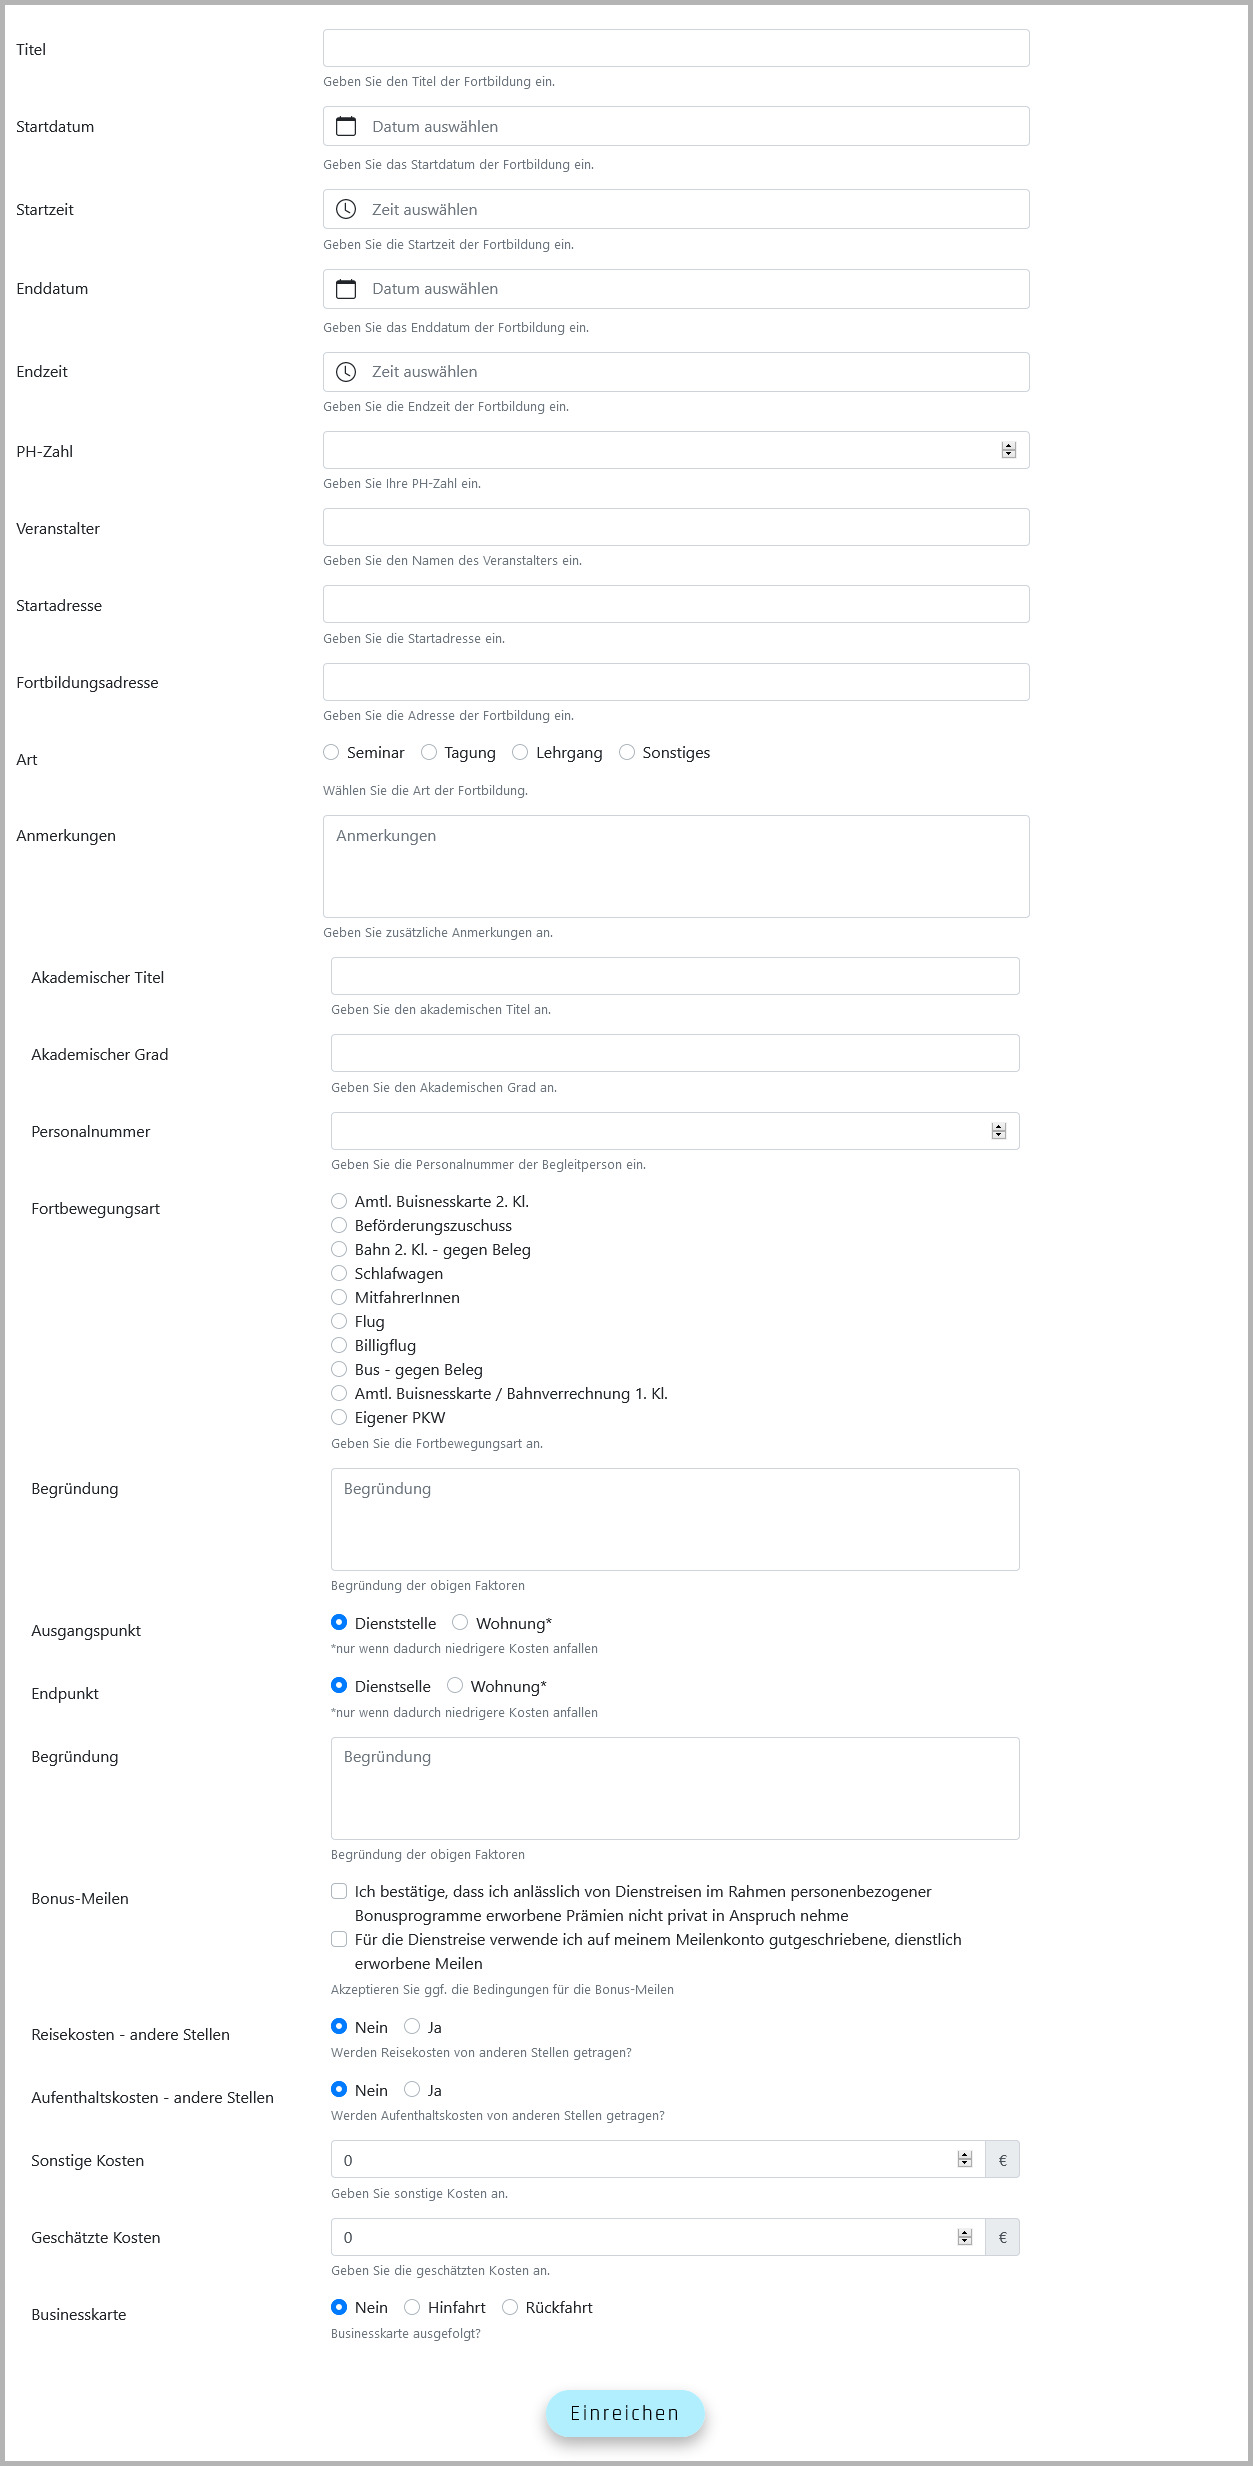
\includegraphics[width=0.63\linewidth]{images/rfoster_implementierung/workshop}
	\caption[Fortbildung]{Eingabefelder einer Fortbildung}
	\label{fig:workshop}
\end{figure}
\newpage
Bei einer Fortbildung kann unterschieden werden, welche Art von Fortbildung erstellt werden soll. Es kann zwischen Seminar, Tagung, Lehrgang und Sonstiges unterschieden werden. Das \textit{JSON}-Objekt wird nach dem Drücken des ''Einreichen''-Knopfes erstellt und mit den angegebenen Daten befüllt. Das Objekt wird anschließend an das Backend gesendet.\\

Das \textit{JSON}-Objekt wird, wie in \autoref{code_submit_data} beschrieben, erstellt. Für eine Fortbildung gibt es nur wenige Änderungen.
Statt dem \textit{SchoolEventDetails}-Objekt wird ein \textit{TrainingDetails}-Objekt in den Antrag hinzugefügt und die Art des Antrags wird auf 1 gesetzt:
\begin{code}{js}
var data = {		// Das JSON-Objekt mit allen Informationen
	Name: this.returnString(this.escorts.description),	// Der Name des Antrags
	Kind: 1,	// Der Typ des Antrags (1 = Fortbildung)
	// ...
	TrainingDetails: {
		Kind: this.returnValue(this.selected),	// Die Art der Fortbildung
		MiscellaneousReason: this.returnString(this.son),	// Falls "Sonstiges" ausgewählt worden ist
		PH: this.returnValue(this.phNumber),	// Die PH Zahl des Lehrers
		Organizer: this.returnString(this.veran)	// Der Veranstalter der Fortbildung
	},
	BusinessTripApplications: business,	// Das Reiseformular für den Lehrer
	TravelInvoices: invoices	// Die Reiserechnung für den Lehrer
};
\end{code}
\captionof{listing}[\textit{JSON} Fortbildung]{\textit{JSON}-Objekt einer Fortbildung}~\\
\newpage
\subsubsection{Sonstiges}
Ein \textit{Sonstiges}-Antrag kann auf der Unterseite ''Anderer Grund'' erstellt werden. Er sieht wie folgt aus und beinhaltet Eingabefelder für alle notwendigen Informationen für den Antrag.
\begin{figure}[H]
	\centering
	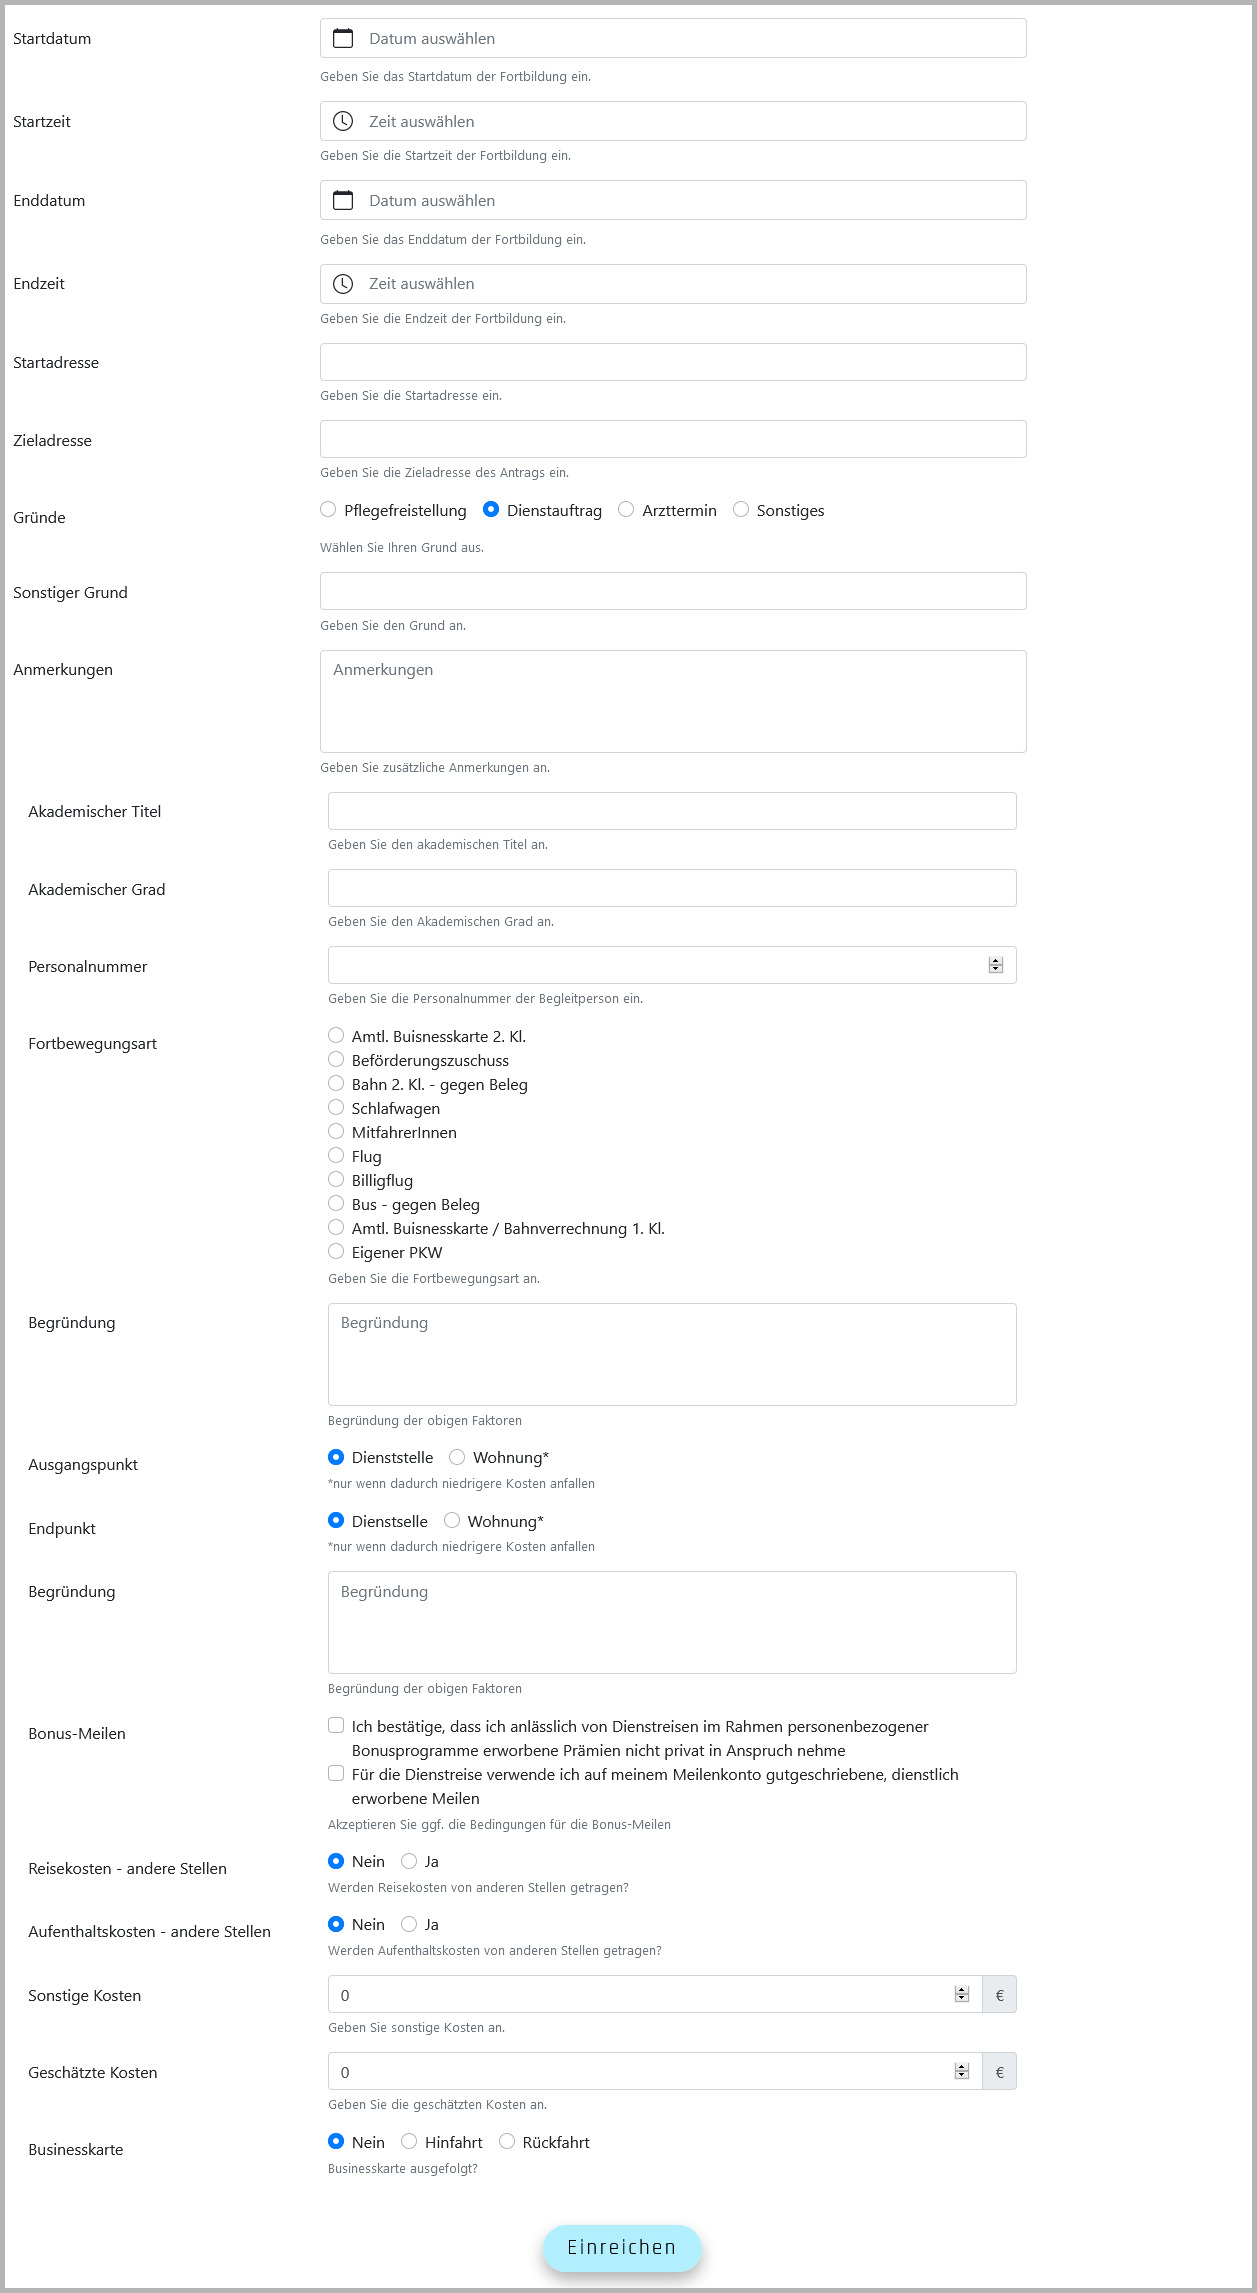
\includegraphics[width=0.6\linewidth]{images/rfoster_implementierung/othercause}
	\caption[Sonstiges Antrag]{Eingabefelder für \textit{Sonstiges}-Antrag}
	\label{fig:othercause}
\end{figure}
\textit{Sonstiges}-Anträge werden unterschieden in Pflegefreistellungen, Dienstaufträge, Arzttermine und Sonstiges. Das \textit{JSON}-Objekt wird nach dem Drücken des ''Einreichen''-Knopfes erstellt und mit den angegebenen Daten befüllt. Das Objekt wird anschließend an das Backend gesendet.\\

Das \textit{JSON}-Objekt wird so erstellt, wie in \autoref{code_submit_data} beschrieben. Für einen \textit{Sonstiges}-Antrag gibt es nur wenige Änderungen.
Statt dem \textit{SchoolEventDetails}-Objekt wird ein \textit{OtherReasonDetails}-Objekt in den Antrag hinzugefügt und die Art des Antrags wird auf 6 gesetzt:
\begin{code}{js}
var data = {		// Das JSON-Objekt mit allen Informationen
	Name: this.returnString(this.escorts.description),	// Der Name des Antrags
	Kind: 6,	// Der Typ des Antrags (6 = Sonstiges Antrag)
	// ...
	OtherReasonDetails: {
		Kind: this.returnValue(this.selected),	// Die Art des Sonstigen Antrags
		MiscellaneousReason: this.returnString(this.son),	// Falls "Sonstiges" ausgewählt worden ist
		ServiceMandateGZ: this.returnValue(this.gz),	// Die GZ des Dienstauftrags
		ServiceMandateTitle: this.returnString(this.title)	// Titel des Dienstauftrags
	},
	BusinessTripApplications: business,	// Das Reiseformular für den Lehrer
	TravelInvoices: invoices	// Die Reiserechnung für den Lehrer
};
\end{code}
\captionof{listing}[\textit{JSON} \textit{Sonstiges}-Antrag]{\textit{JSON}-Objekt eines \textit{Sonstiges}-Antrags}~\\
\subsubsection{Antrag einreichen}
Sobald der Benutzer auf den "Einreichen"-Knopf drückt, wird das \textit{JSON}-Objekt erstellt und an das Backend gesendet. Dies erfolgt mit folgendem Code:
\begin{code}{js}
	axios.post(this.url + "/createApplication", // Es wird eine createApplication-Anfrage an das Backend gesendet
	{
		headers: {
			Authorization: "Basic " + this.token
		}
	},
	data // Der Antrag mit den eingegebenen Daten wird mit der Anfrage gesendet
	)
\end{code}
\captionof{listing}[Antrag einreichen]{Beispiel um einen Antrag im Backend zu erstellen}~\\
\newpage
\subsection{Antrag Ansicht}
\label{sec:antrag_ansicht}
Wenn die Unterseite, die einen Antrag anzeigen soll, geladen wird, so wird der Unterseite die ID des Antrags mitgegeben. Sobald die Komponente geladen wird, wird mit dieser ID eine Anfrage an das Backend gesendet, um den gesamten Antrag zu laden. Die Informationen werden interpretiert und angezeigt.
\subsubsection{Fortschrittsanzeige}
Jeder Antrag besitzt einen Fortschritt, welcher graphisch durch eine \textit{Progress}-Komponente angezeigt wird. Die Komponente erhält von der \textit{Antrag-Ansicht} den Fortschritt des Antrags und die Art des Antrags als Nummer, um die Informationen für den Benutzer lesbar anzuzeigen.
\begin{figure}
	\centering
	
\includegraphics[width=1\linewidth]{images/rfoster_implementierung/progress}
	\caption[Fortschrittsanzeige]{Fortschrittsanzeige für einen Antrag}
	\label{fig:progress}
\end{figure}
\subsubsection{Dokumente}
In einem Antrag werden mehrere Dokumente gespeichert. Die Dokumente können je nach Fortschritt des Antrags bearbeitet werden und werden in einer Liste angezeigt:
\begin{figure}
	\centering
	
\includegraphics[width=1\linewidth]{images/rfoster_implementierung/documents}
	\caption[Dokumente eines Antrags]{Die Dokumente einer Schulveranstaltung}
	\label{fig:documents}
\end{figure}

Folgende Dokumente werden je nach Antragsart erstellt:
\paragraph{Schulveranstaltung}~\\
Die Schulveranstaltung besitzt zwei Dokumente: zum Einen die allgemeinen Informationen zu der Veranstaltung und zum Anderen die Informationen zu den Begleitpersonen.
\begin{itemize}
	\item \textbf{Allgemeine Informationen}\\
	In diesem Dokument werden generelle Informationen über die Schulveranstaltung gespeichert. Diese können nur von dem Leiter des Antrags eingesehen und bearbeitet werden.
	\item \textbf{Informationen zu Begleitlehrern}\\
	In diesem Dokument sieht jeder Begleitlehrer sein eigenes Formular, welches er je nach Fortschritt des Antrags bearbeiten kann. In diesem Dokument werden Informationen über die An- und Abreise sowie den Aufenthalt des Lehrers gespeichert.
\end{itemize}
\newpage~
\paragraph{Fortbildung}~\\
In einem Fortbildungsformular werden Informationen über die Fortbildung und den Lehrer gespeichert.
\paragraph{Sonstiges}~\\
In einem \textit{Sonstiges}-Antrag werden Informationen über den Grund des Antrags sowie den Zeitraum gespeichert.
\paragraph{Reiseformular}~\\
Ein Reiseformular wird bei den meisten Arten von Antrag erstellt. In einem Reiseformular werden Informationen über den Lehrer und über dessen An- und Abreise gespeichert.
\paragraph{Reiserechnung}~\\
Eine Reiserechnung wird bei den meisten Arten von Antrag erstellt. In einer Reiserechnung werden Informationen über die Kosten des Antrags gespeichert und wie diese entstanden sind. Des weiteren können Belege hochgeladen werden, um diese dem Antrag zu hinterlegen. Ein Beleg wird mit folgendem Code hochgeladen:
\begin{code}{js}
	axios.post(this.url + "/saveBillingReceipt",
	{
		params: {
			uuid: this.app.uuid, // Der Antrag wird spezifiziert, für den die Belege hochgeladen werden
			shortname: this.user.short // Es wird der Lehrer spezifiziert, der die Belege hochlädt
		}
	},
	{
		headers: {
			Authorization: "Basic " + this.token
		}
	},
	belege // Die Belege, welche hochgeladen werden
	)
\end{code}
\captionof{listing}[Belege hochladen]{Beispiel um Belege hochzuladen}~
\newpage
\subsubsection{Aktionen}
\paragraph{Excel herunterladen}~\\
Der Benutzer kann Reiseformulare und Reiserechnungen als Excel-Datei herunterladen. Diese werden mit folgendem Code erstellt und heruntergeladen \cite{down_excel}:
\begin{code}{js}
	var anchor_href =
	"data:application/vnd.openxmlformats-officedocument.spreadsheetml.sheet;base64," +
	excel;	// Wandelt die Daten vom Backend in eine Excel-Datei um
	var exportLinkElement = document.createElement("a");
	
	exportLinkElement.hidden = true;
	exportLinkElement.download = "Formular.xlsx";
	exportLinkElement.href = anchor_href;
	exportLinkElement.text = "downloading...";
	
	document.body.appendChild(exportLinkElement);
	exportLinkElement.click();
	exportLinkElement.remove();
\end{code}
\captionof{listing}[Excel Download]{Excel erstellen und herunterladen}~\\
\paragraph{PDF öffnen}~\\
Der Benutzer kann die PDFs der Dokumente öffnen. Die PDFs werden in einem neuen Tab im Browser angezeigt.\\
Mit folgendem Code wird eine PDF erstellt und in einem neuen Tab geöffnet \cite{sof_pdf}:
\begin{code}{js}
	let pdfWindow = window.open("");
	var fileName = "PDF";
	pdfWindow.document.write(
	"<html<head><title>" +
	fileName +
	"</title><style>body{margin: 0px;}iframe{border-width: 0px;}</style></head>"
	);
	pdfWindow.document.write(
	"<body><embed width='100\%' height='100\%' src='data:application/pdf;base64, " +
	encodeURI(pdf) +
	"#toolbar=0\&navpanes=0\&scrollbar=0'></embed></body></html>"
	);
\end{code}
\captionof{listing}[PDF erstellen und öffnen]{PDF erstellen und öffnen im Browser}~
\newpage
\paragraph{Änderungen speichern}~\\
Der Benutzer kann die Änderungen eines Antrags speichern. Dies kann in bestimmten Phasen eines Antrags geschehen. Die Änderungen werden an das Backend gesendet, sobald auf den ''Änderungen Speichern''-Knopf gedrückt wird. Das senden erfolgt mit folgendem Code:
\begin{code}{js}
	if (this.belege.length >= 1) {
		this.sendReceipts(this.belege); // Falls Belege angegeben worden sind, werden diese hochgeladen
	}
	if (this.checkProgression()) {
		this.app.progress = 2;	// Falls alle Begleitlehrer ihre Reiseformulare ausgefüllt haben, wird der Fortschritt auf den nächsten Schritt gesetzt
	}
	if (this.checkInvoices()) {
		this.app.progress = 6; // Falls alle Begleitlehrer ihre Reiserechnungen ausgefüllt haben, wird der Fortschritt auf den nächsten Schritt gesetzt
	}
	this.app.last_changed = this.createNewDate(); // Das Datum der letzten Änderung wird im Antrag gespeichert.
	axios.put(this.url + "/updateApplication?uuid=" + this.app.uuid,
	{
		headers: {
			Authorization: "Basic " + this.token
		}
	},
	this.app // Es wird der neue Antrag (Mit den neuen Änderungen) hochgeladen
	)
\end{code}
\captionof{listing}[Antrag speichern]{Beispiel um die Änderungen eines Antrags zu speichern}~\\
\paragraph{Antrag schließen}~\\
Der Leiter eines Antrags kann den Antrag schließen. Sobald der Antrag geschlossen ist, wird dieser im Backend auf den Fortschritt abgeschlossen gesetzt. Dies wird mit folgendem Code erreicht:
\begin{code}{js}
	if (this.app.kind === 0) {	// Der Fortschritt wird je nach Antragsart auf Abgeschlossen gesetzt
		this.app.progress = 7;
	} else {
		this.app.progress = 6;
	}
	this.save(); // Der Antrag wird gespeichert
	this.hideClose(); // Das Modal wird geschlossen
\end{code}
\captionof{listing}[Antrag schließen]{Beispiel um einen Antrag zu schließen}~\\
\newpage
\paragraph{Antrag löschen}~\\
Der Leiter eines Antrags kann den Antrag löschen. Sobald auf den Knopf ''Antrag löschen'' gedrückt wird, wird dieser im Backend gelöscht. Der Benutzer wird daraufhin weitergeleitet auf die Startseite. Ein Antrag wird mit folgender Anfrage gelöscht:
\begin{code}{js}
	axios.delete(this.url + "/deleteApplication?uuid=" + this.app.uuid, { // Es wird ein Delete-Request an das Backend gesendet
		headers: {
			Authorization: "Basic " + this.token
		}
	})
\end{code}
\captionof{listing}[Antrag löschen]{Beispiel um einen Antrag zu löschen}~\\
\newpage
\subsection{Antrag Übersicht}
\label{sec:antrag_uebersicht}
Um einen Überblick über die Anträge zu haben, gibt es zwei Übersichtsseiten, welche die Anträge auflisten. In den Auflistungen sieht man die groben Daten des Antrags und kann diese in der \textit{Antrag-Ansicht} öffnen. Sobald eine Übersichtsseite aufgerufen wird, werden die Anträge abgefragt und in einer Liste angezeigt:
\begin{figure}[H]
	\centering
	
\includegraphics[width=1\linewidth]{images/rfoster_implementierung/liste_antrag}
	\caption[Liste der Anträge]{Auflistung von Anträgen auf der Übersichtsseite}
	\label{fig:listeantrag}
\end{figure}

\subsubsection{Alle Anträge}
Auf dieser Übersichtsseite werden alle Anträge angezeigt, die mit dem angemeldeten Benutzer zusammenhängen.
\subsubsection{Aktive Anträge}
In der Auflistung der aktiven Anträge, werden alle Anträge angezeigt, welche nicht abgeschlossen sind. Ist nur ein Antrag in der Liste der aktiven Anträge, so wird der Antrag sofort in der \textit{Antrag-Ansicht} geöffnet.
\subsubsection{Aktionen}
\paragraph{Schnelle Informationen}~\\
Wird auf den Knopf ''Schnelle Informationen'' gedrückt, öffnet sich ein Fenster, in dem die groben Informationen des Antrags angezeigt werden.
\paragraph{Antrag betrachten}~\\
Wird auf den Knopf ''Antrag betrachten'' gedrückt, wird der Antrag in der \textit{Antrag-Ansicht} geöffnet.
\newpage
\subsection{Administrator}
\subsubsection{Antrag Ansicht}
Der Aufbau der \textit{Antrag-Ansicht} ähnelt dem aus \autoref{sec:antrag_ansicht}.\\
Ein Administrator kann alle Informationen eines Antrags einsehen und diesen akzeptieren. Des Weiteren können alle PDFs des Antrags geöffnet werden. Der Antrag kann auch abgelehnt werden, wodurch der Fortschritt zurückgesetzt wird. Wenn der Antrag abgelehnt wird, kann ein Grund für das Ablehnen angegeben werden. Der Antragsteller kann daraufhin die Informationen des Antrags aktualisieren und damit den Antrag erneut einreichen oder den Antrag schließen.
\subsubsection{Antrag Übersicht}
Die Übersichtsseite für Administratoren ähnelt dem Aufbau aus \autoref{sec:antrag_uebersicht}.\\
Der Administrator sieht, wer den Antrag gestellt hat, und kann mehrere Anträge auswählen, um diese in einer PDF anzuzeigen.
Des Weiteren kann auf den Knopf ''Antrag betrachten'' gedrückt werden, wodurch der Administrator auf die Antrag Ansicht für Administratoren weitergeleitet wird.
\newpage
\subsubsection{Rechte}
Die Rechte für Benutzer können über ein Formular bearbeitet werden. Die E-Mail-Adresse des zu bearbeitenden Nutzers wird in dem Formular angegeben. Zusätzlich werden über die Auswahl die Rechte von dem Benutzer gesetzt.
\begin{figure}[H]
	\centering
	
\includegraphics[width=1\linewidth]{images/rfoster_implementierung/rights}
	\caption[Formular der Rechte]{Formular, um Rechte eines Benutzers zu setzen}
	\label{fig:rightsform}
\end{figure}
Sobald auf den ''Rechte speichern''-Knopf gedrückt wird, wird das Formular ausgelesen und damit die Anfrage für das Backend erstellt. Die Anfrage an das Backend wird folgendermaßen gesendet:
\begin{code}{js}
	axios.get(this.url + "/setTeacherPermissions?uuid=" + response.data.uuid,
	{
		headers: {
			Authorization: "Basic " + this.token
		}
	}, rechte	// Die im Formular eingestellten Rechte
	)
	.then(res => {
		if (res.status === 200) {
			this.saveComplete();
			this.reset();
		}
	});
\end{code}
\captionof{listing}[Anfrage Rechte setzen]{Anfrage zum Setzen der Rechte eines Benutzers}~\\